\section{Advanced Topics on Sinkhorn Algorithm}

During this tour, we dived a bit more into Sinkhorn's algorithm and various adaptation. 

\subsection{Wasserstein Flow for Matching}

There are a few things to say in this section. To begin with, I used the data provided at the beginning of the notebook, ie. $n=200$ points sample on a square for $\alpha$ and $m=100$ points sample on a circle for $\beta$, with uniform weights. The result of the flow, for various values of the regularization parameter $\epsilon$ and at different steps of the gradient descent are shown fig. \ref{fig:wassertein_flows_for_various_eps}. 

\begin{figure}[p]
    \centering
    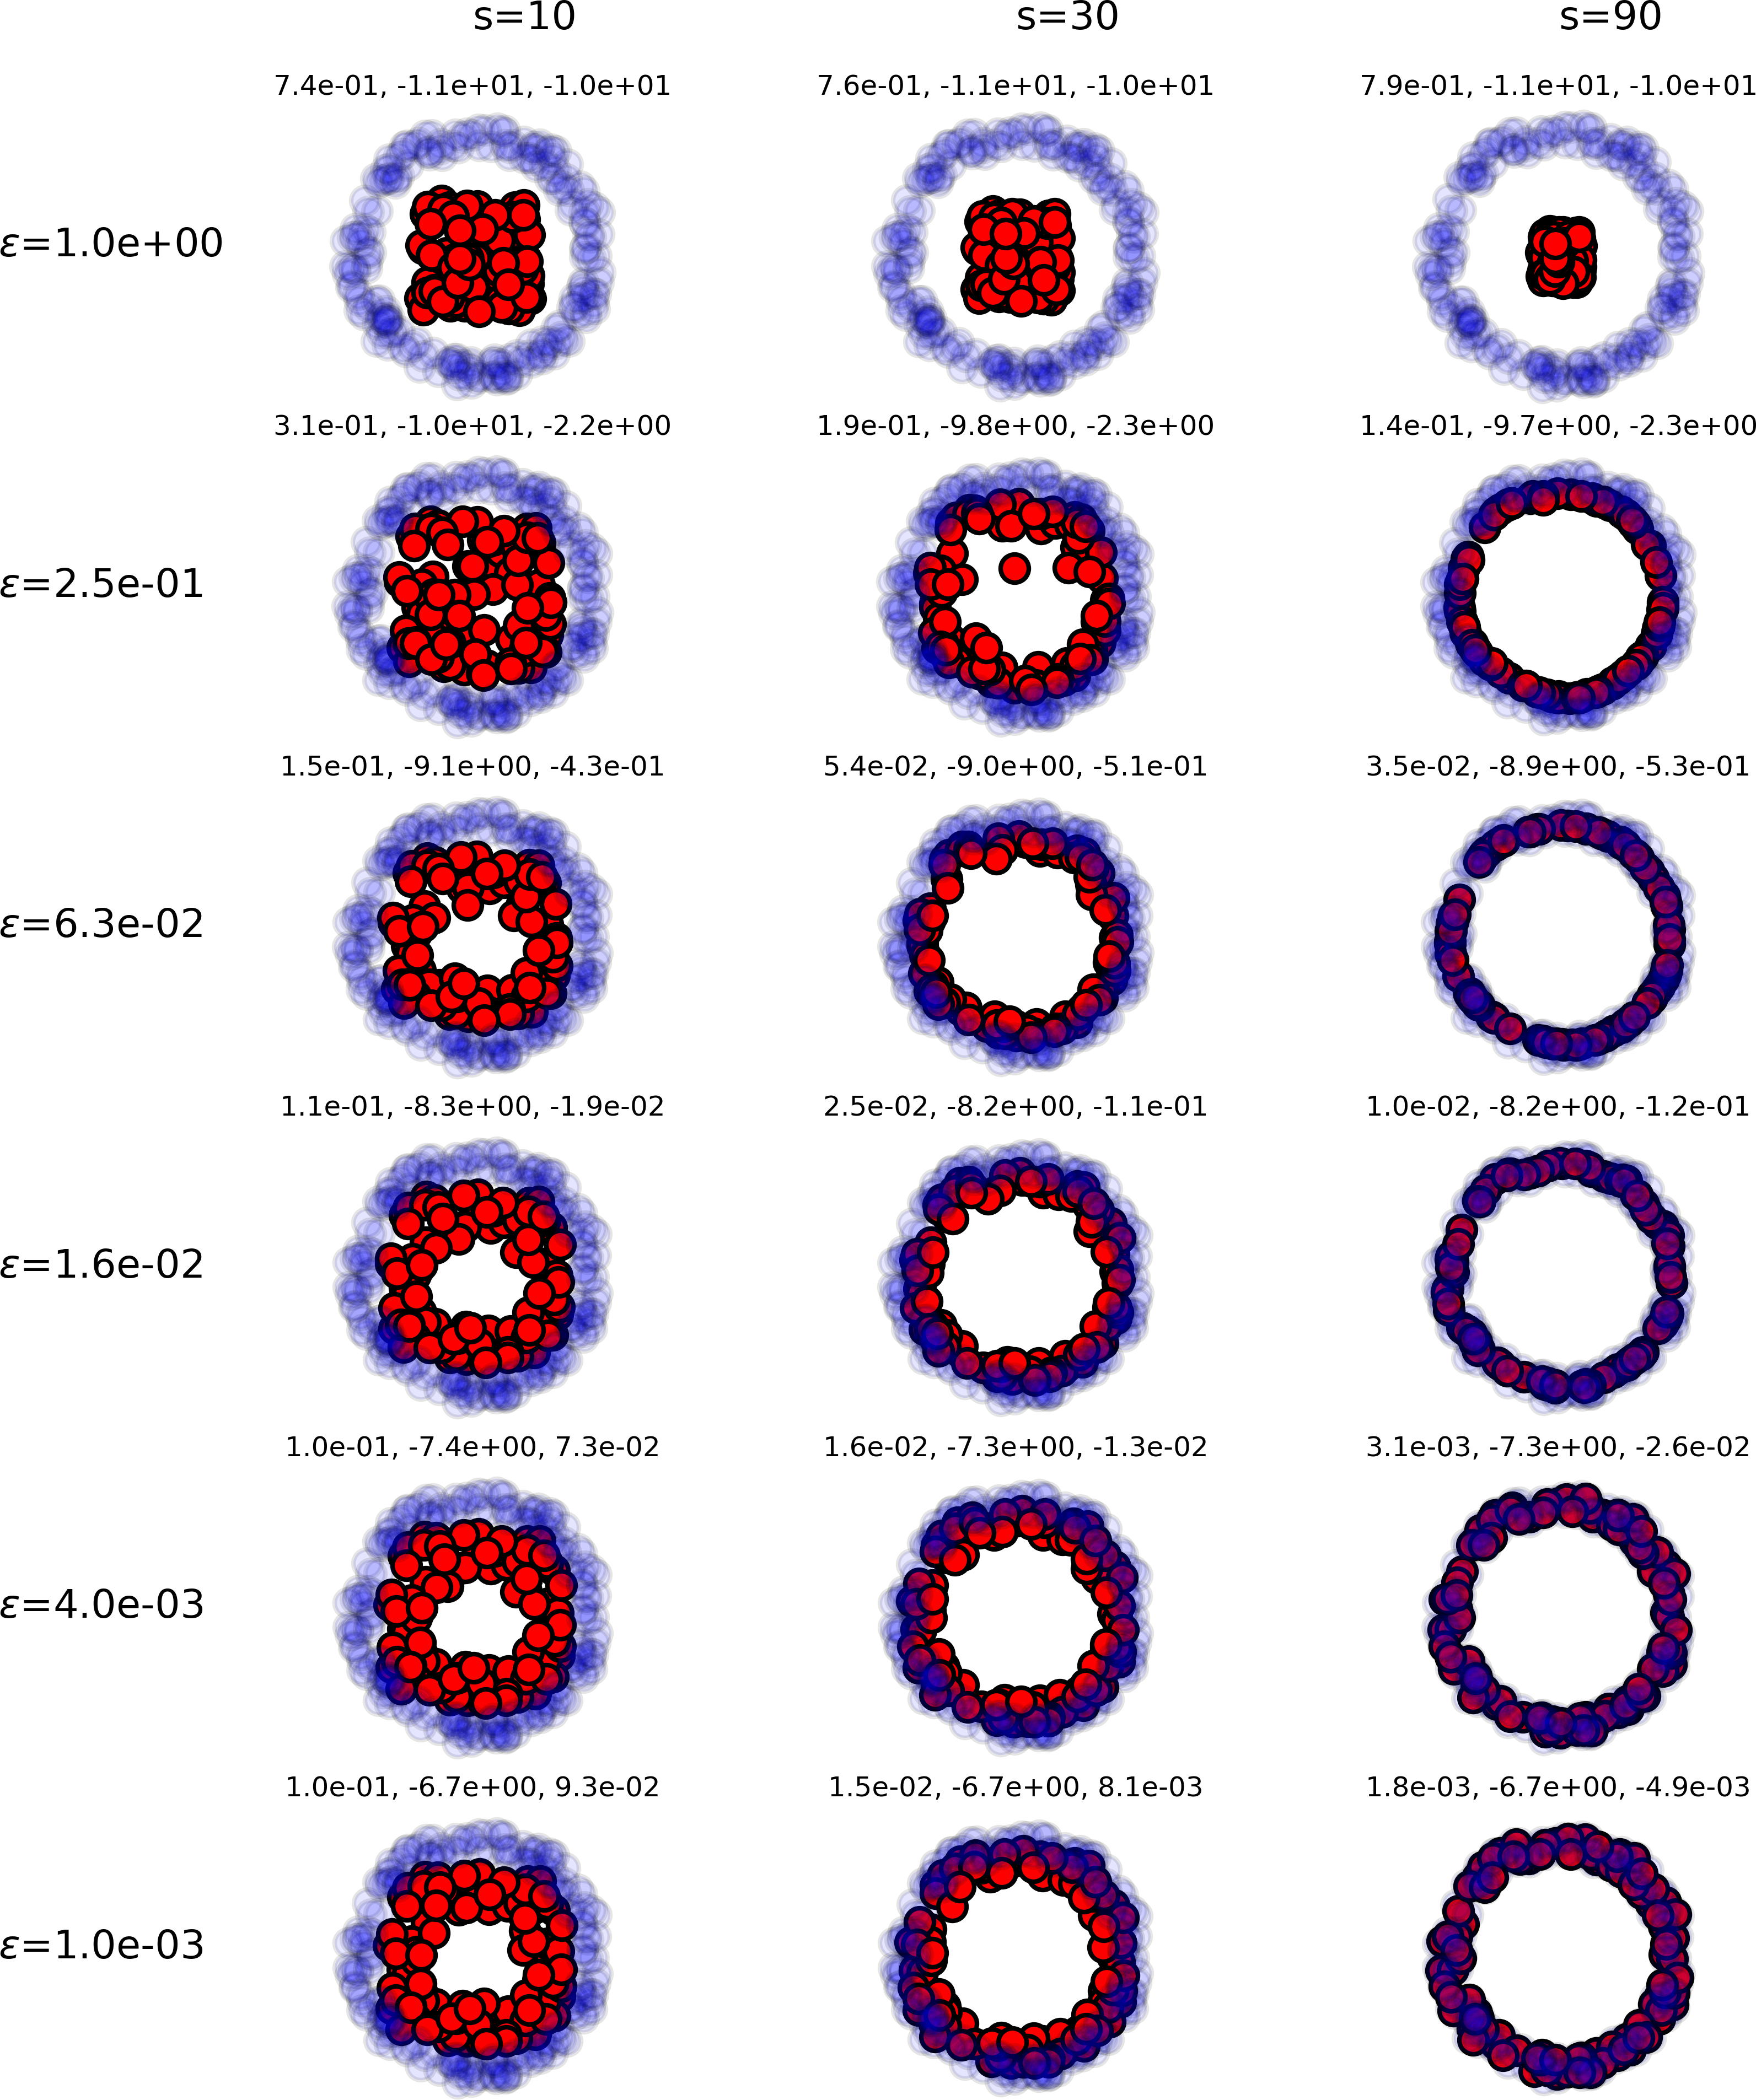
\includegraphics[width=\textwidth]{samples/4/wassertein_flow_for_various_eps.png}
    \caption{Wassertein flow. Rows are sorted with decreasing value of the regularization parameter $\epsilon$. Columns are sorted with increasing values of timesteps during the descent. Above each plot is indicated the \textbf{energy} of the current $z$: first the trace, then the entropy, then the weighted sum of both with $(1, \epsilon)$. The best trace term is achieved with the lowest $\epsilon$, at the end of the descent. The maximum entropy is reached with the biggest $\epsilon$. During all simulation, the step size is set to $\tau=0.5$. It seems too much for $\epsilon=1$}
    \label{fig:wassertein_flows_for_various_eps}
\end{figure}

\paragraph{Results} A few things to say about the results:
\begin{itemize}
    \item It seems that the bigger $\epsilon$, the smaller the the step size for the gradient descent should be. That, or there is a \textbf{threshold} effect on $\epsilon$, aboce which the entropy term always wins at the expense of the trace term.
    \item Below that threshold, it seems that all distribution seem to converge well. As expected, if one wants a \textbf{precise} final result, one needs to \textbf{lower} $\epsilon$ accordingly.
\end{itemize}

Finally, I plot the final score (at the end of the gradient descent) to see the contribution of the trace and of the entropy. Result is fig. \ref{fig:score_epsilon_wassertein_flow}.

\begin{figure}[p]
    \centering
    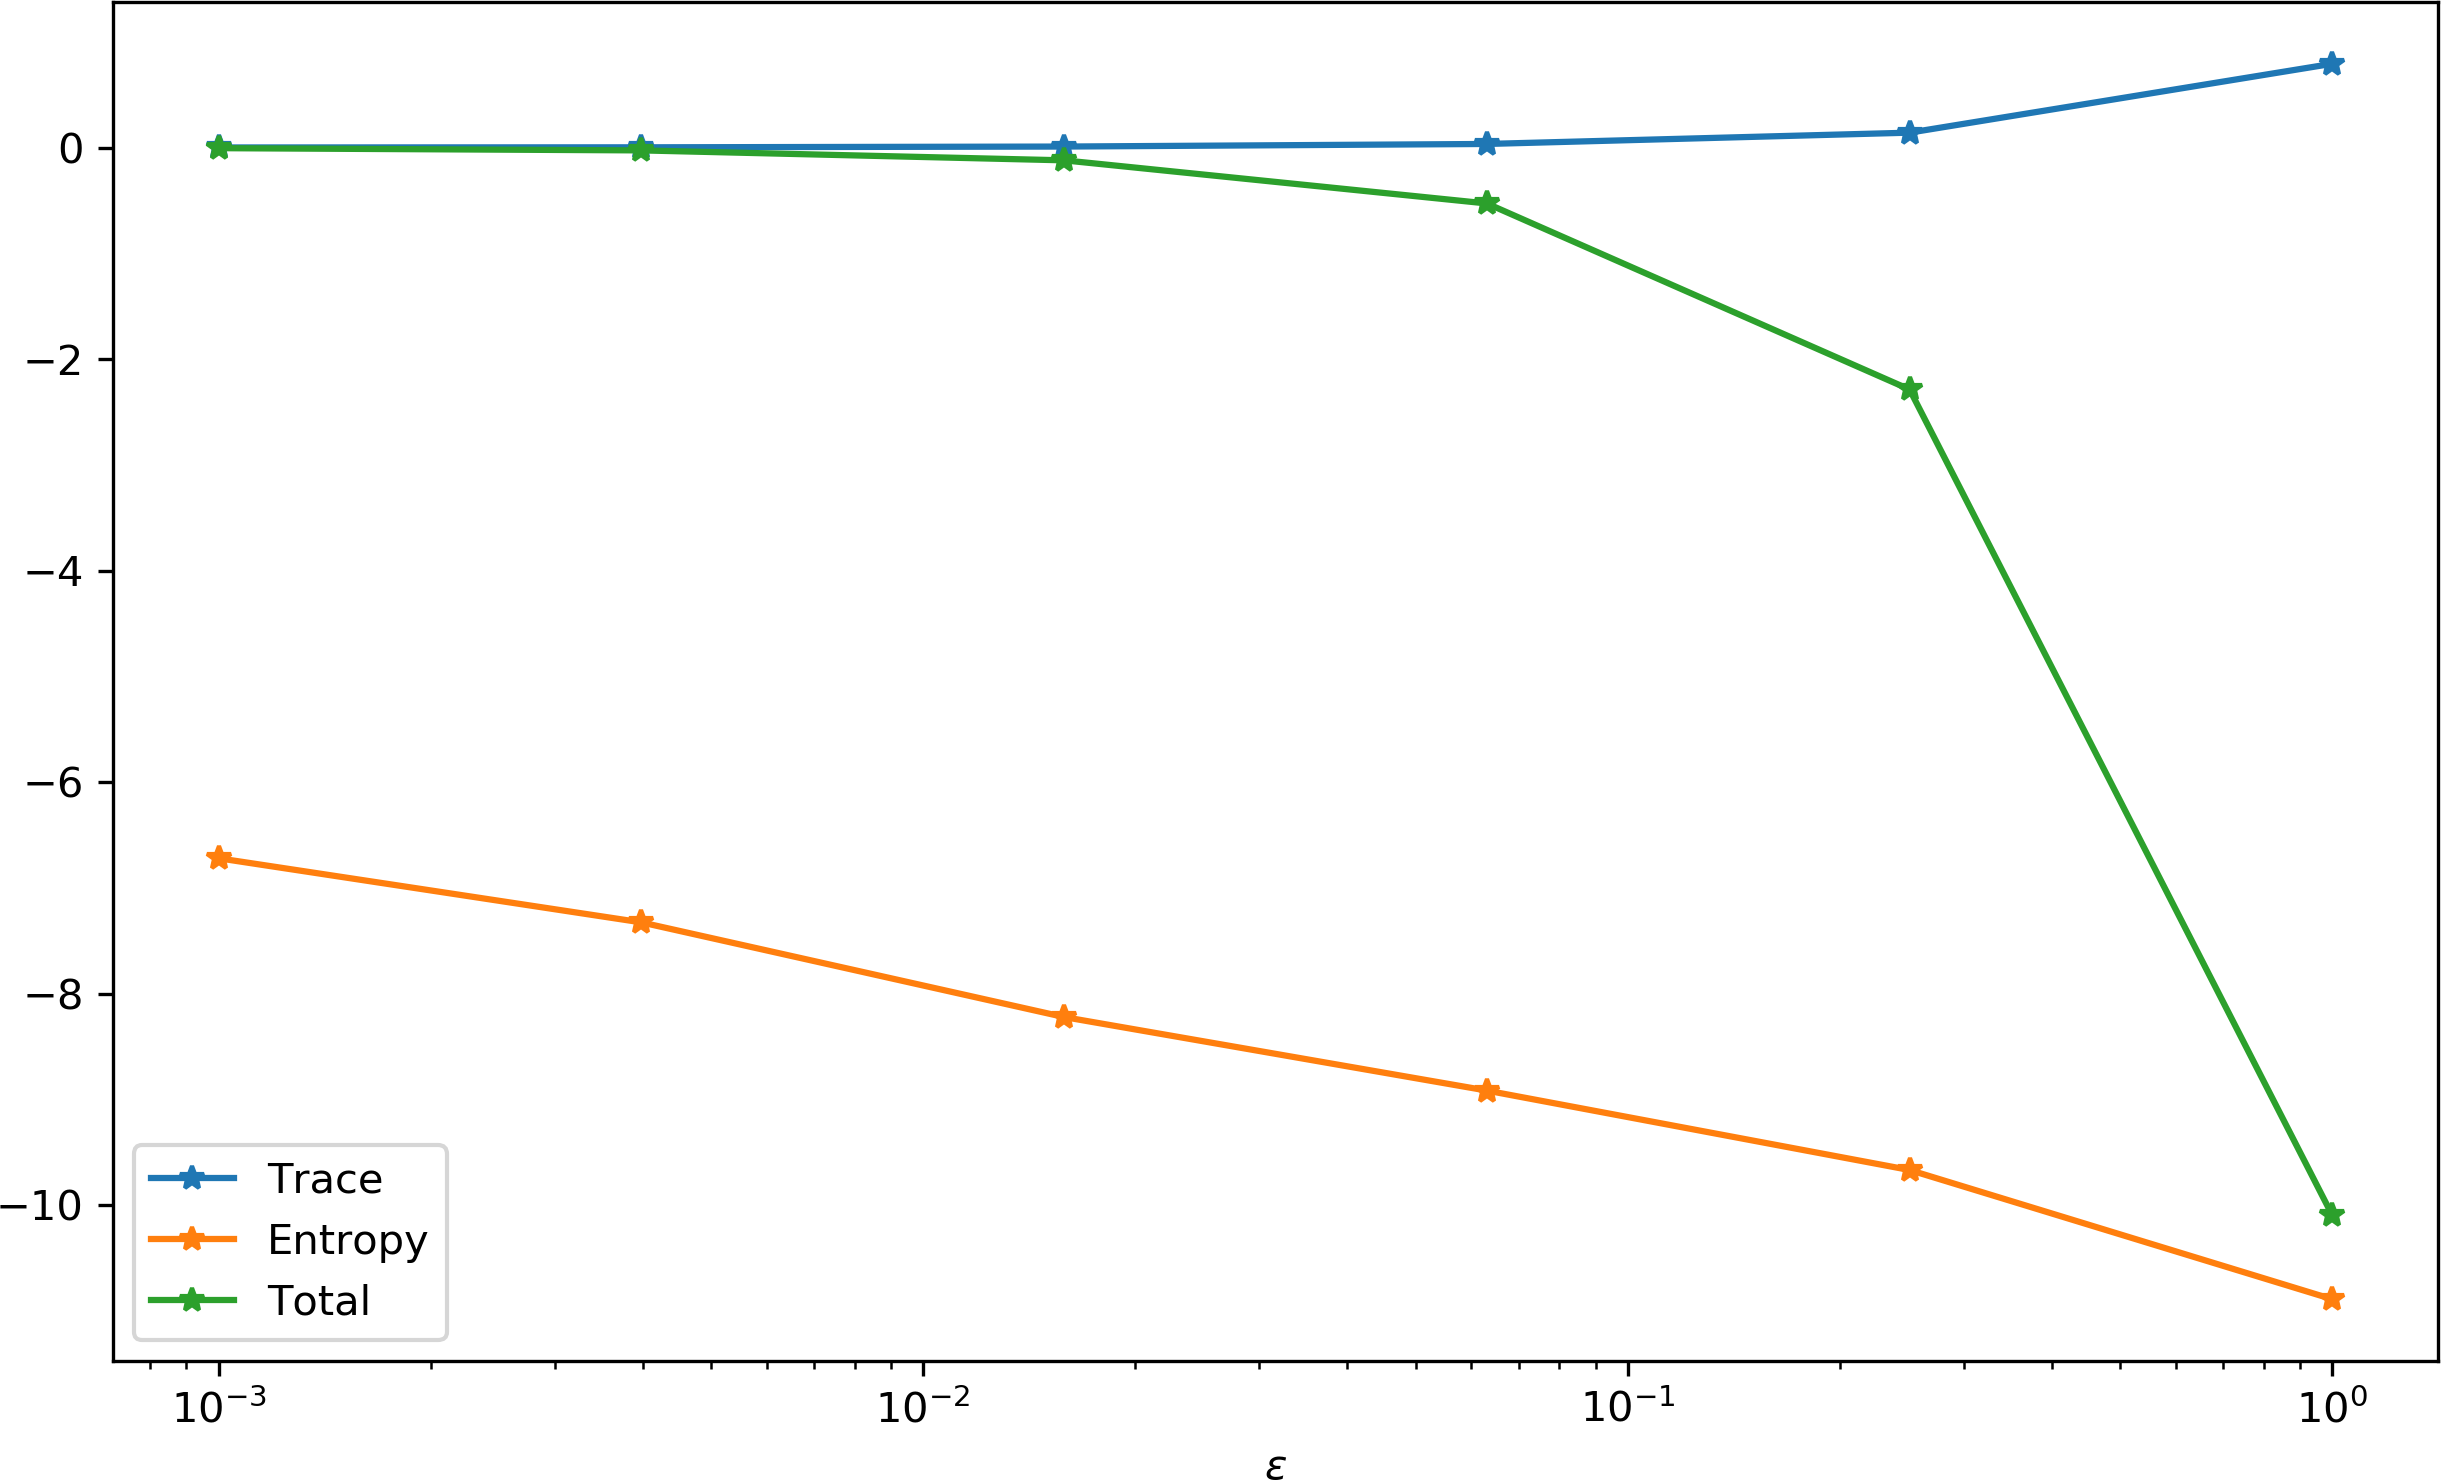
\includegraphics[width=.7\textwidth]{samples/4/evolution_of_score_epsilon.png}
    \caption{Value of the energy at the end of the descent. As $\epsilon$ grows, the entropy weight more and more in the energy term. When it is small, we are the closest to our objective.}
    \label{fig:score_epsilon_wassertein_flow}
\end{figure}

\paragraph{Execution time} The implementation did not posed any difficulties, except for a surprising result. Below, on table \ref{tab:execution_time}, I show the execution time for the multiple gradient descents.

\begin{table}[h]
\centering
\begin{tabular}{cc}
$\epsilon$    & $t$ (s) \\
\hline
$1.0$         & $21$    \\
$2.5 \, 10^{-1}$ & $25.3$  \\
$6.3 \, 10^{-2}$ & $27.8$  \\
$1.6 \, 10^{-2}$ & $23.7$  \\
$4.0 \, 10^{-2}$ & $85.1$  \\
$1 \, 10^{-3}$   & $259.1$
\end{tabular}
\caption{Execution time of the Wassertein flow for various values of $\epsilon$. Each run used $100$ gradient steps, and each used $200$ Sinkhorn steps to compute the optimal transport plan $P$. The time should be roughly constant, as complexity does not depend of $\epsilon$.}
\label{tab:execution_time}
\end{table}

At first, I thought: "totally fine: the smaller $\epsilon$, the sparser the solution and the greater the computation time". However, each gradient step uses a \textbf{fixed} number of Sinkhorn steps. The stopping criteria is not about tolerance. Thus, this result was really surprising. 

After looking up the code through and through, it is in fact due to a kind of exotic issue: it has to do with Numpy's \texttt{exp} function. Looking at the source code, it appears the computations work in two ways:
\begin{enumerate}
    \item First, look up the values in a table, and compute the rest with the desired precision.
    \item If that does not give a sufficient precision, it falls back on a classical Taylor expansion computation.
\end{enumerate}

In fact, it appears it is exactly the problem we are facing here. To be sure, I computed $x\mapsto e^{x/\epsilon}$ for $10000$ values of $x$ between 0 and 1, and recorded the computation time. The result is shown fig. \ref{fig:exponential_computation_time}.

\begin{figure}[b]
    \centering
    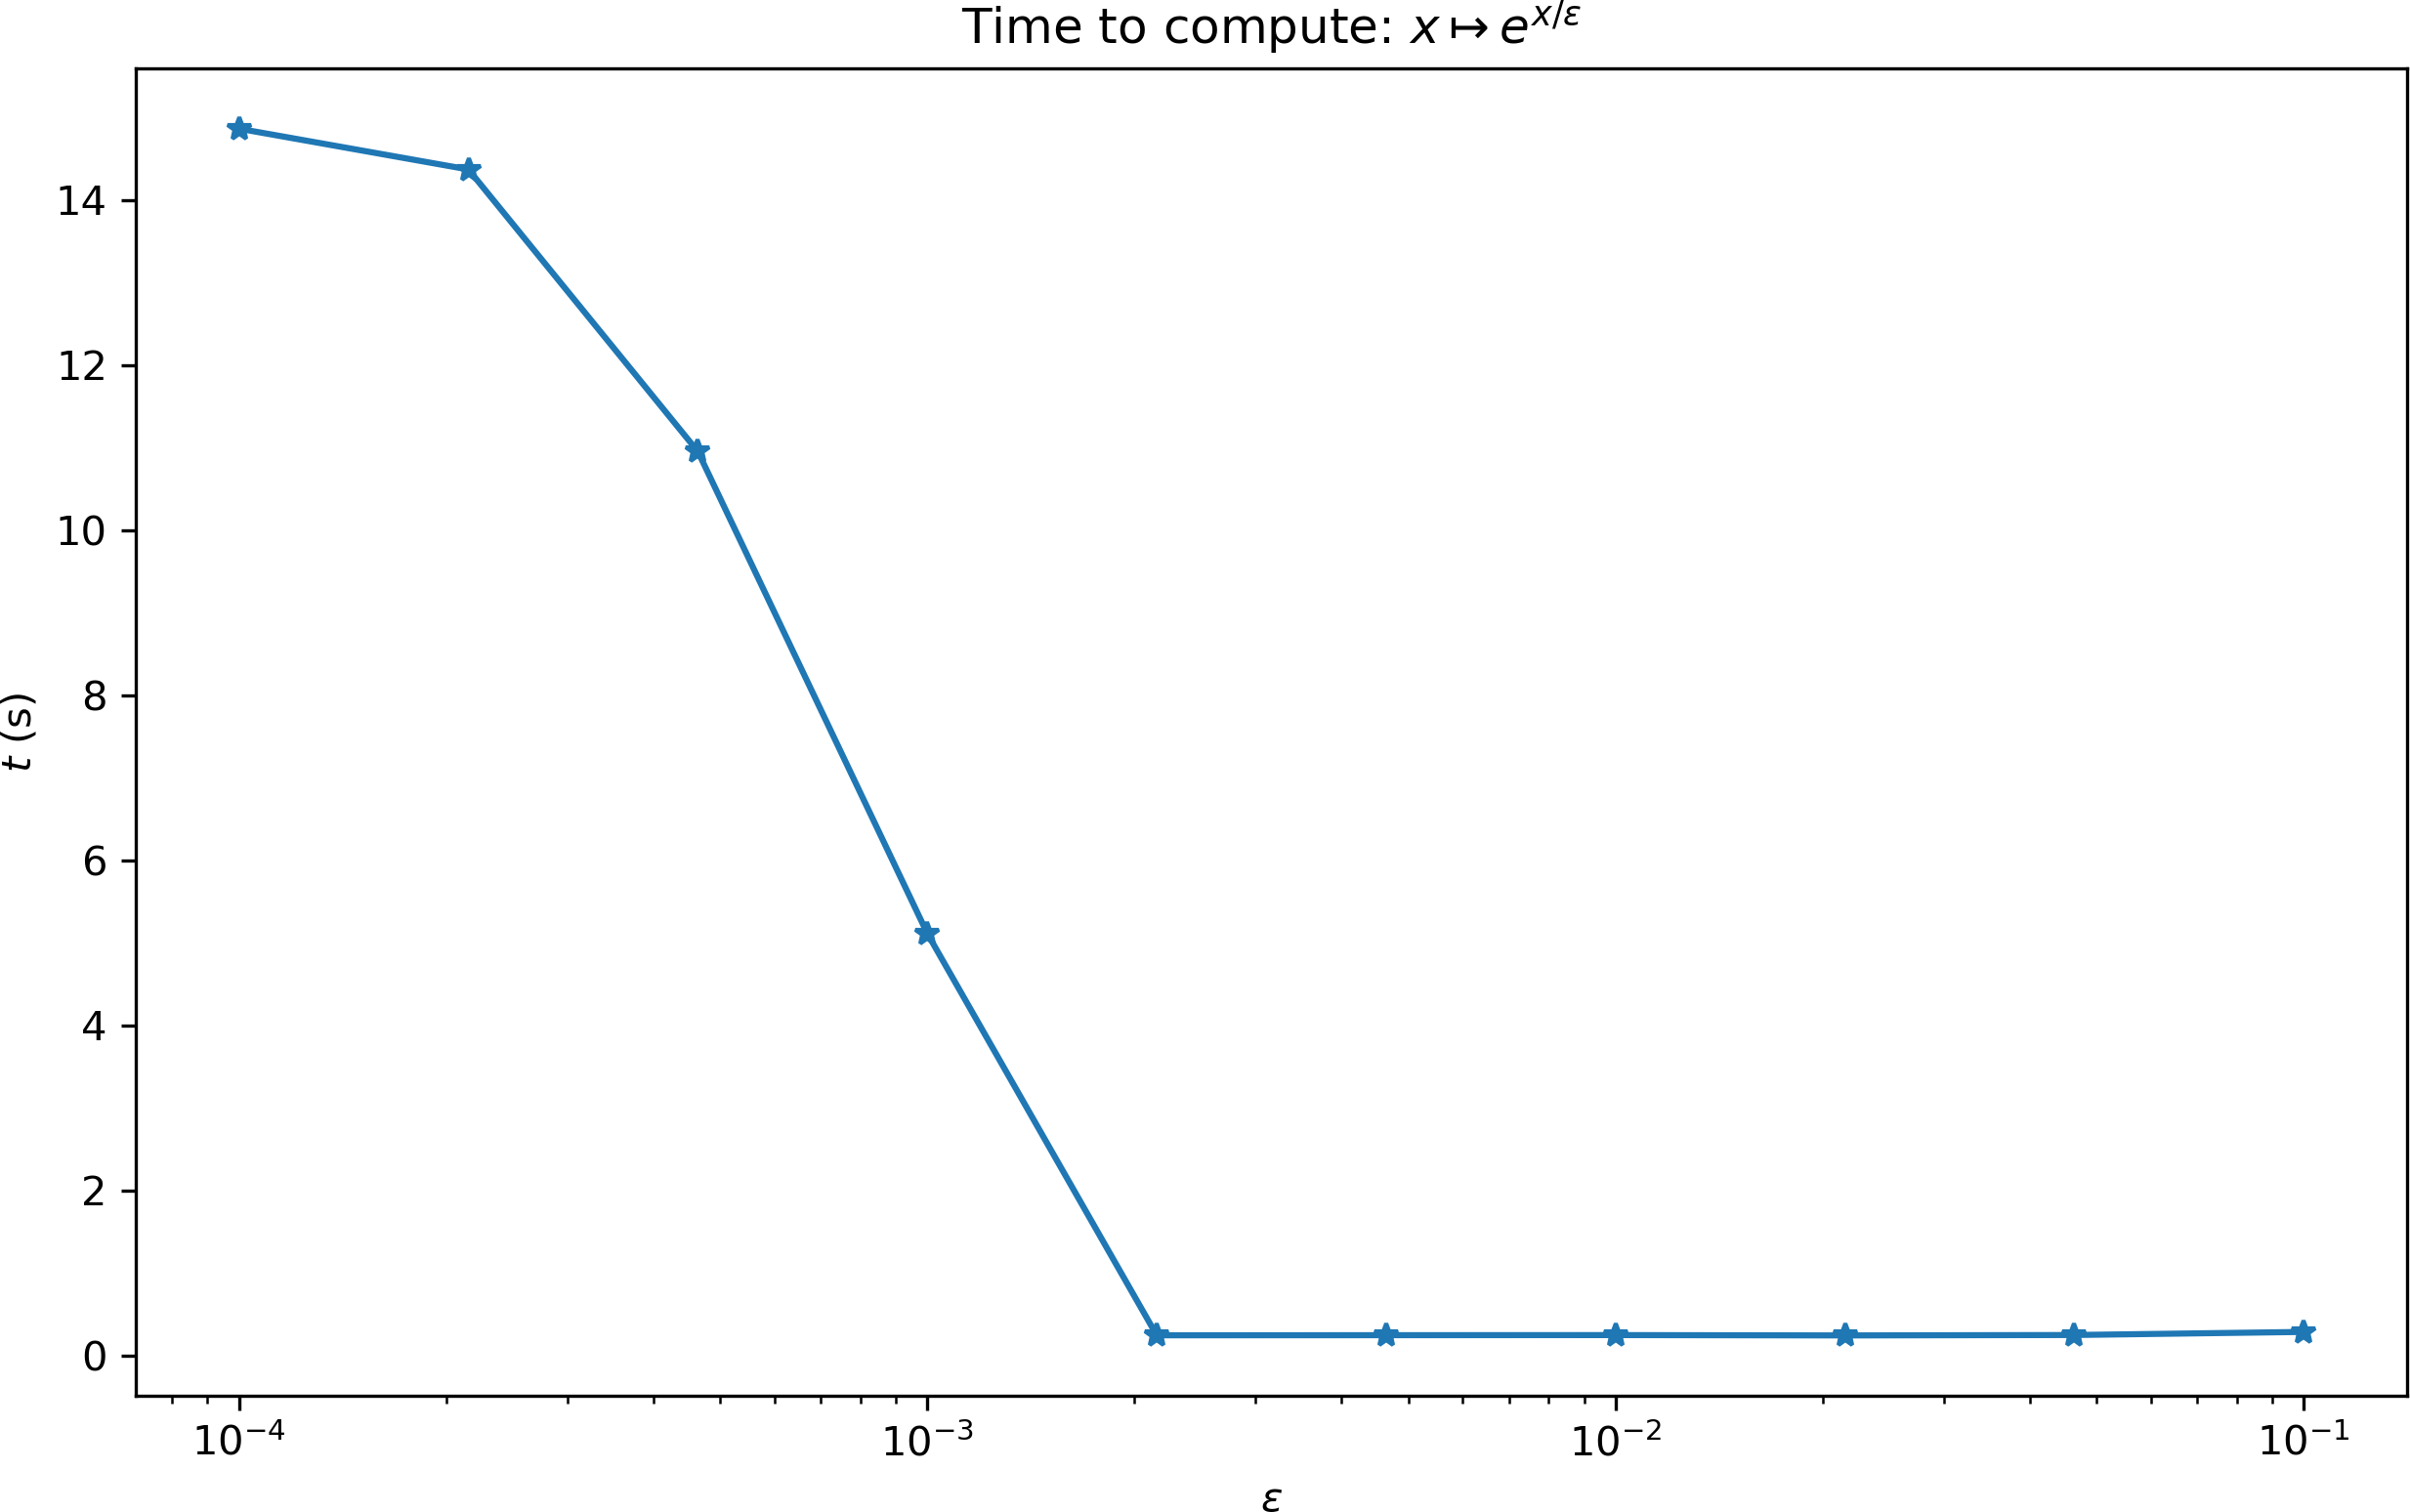
\includegraphics[width=.7\textwidth]{samples/4/exponential_computation_time.png}
    \caption{Execution time of $x \mapsto e^{x/\epsilon}$ for $10000$ values of $x$ between 0 and 1, function of $\epsilon$. If its value is too small, Numpy computes a Taylor expansion which greatly increases the computation time.}
    \label{fig:exponential_computation_time}
\end{figure}

It is purely a numerical issue. Yet, it can be very annoying in our case, with a factor $10$ in the computation time between for $\epsilon>10^{-3}$ and smaller values. 

